%%%%%%%%%%%%%%%%%%%%%%%%%%%%%%%%%%%%%%%%%%%%%%%%%%%%%%%%%%%%%%%%%%%%%%%%%%%%%%%%
\talkpart{1}{The Basics}
%%%%%%%%%%%%%%%%%%%%%%%%%%%%%%%%%%%%%%%%%%%%%%%%%%%%%%%%%%%%%%%%%%%%%%%%%%%%%%%%
% --- SLIDE ---
\begin{frame}[fragile]
\frametitle{LLDB - Architecture}  

\hspace{10pt}
\hspace{50pt}
\begin{tikzpicture}
  \node[draw=uipurple,rounded corners = 1pt, fill=uidarkgray,text=white, line width=1.5pt, minimum width = 2cm, minimum height = 1.25cm] (lldb) at (15,3) {lldb};
  \node[draw=uipurple,rounded corners = 1pt, fill=uidarkgray,text=white, line width=1.5pt, minimum width = 3cm, minimum height = 1.25cm] (usr-driver) at (20,3) {user driver};
  \node[draw=uipurple,rounded corners = 1pt, fill=uidarkgray,text=white, line width=1.5pt, minimum width = 3cm, minimum height = 1.25cm] (hw-driver) at (20,0) {debug API};
  \node[draw=uipurple,rounded corners = 1pt, fill=uidarkgray,text=white, line width=1.5pt, minimum width = 2cm, minimum height = 1.25cm] (lldb-server) at (15,0) {lldb-server};
  
  \draw[<->] (lldb) to (usr-driver) [line width=1pt];
  \draw[->] (lldb) to node[midway, right, text width = 2cm] {TCP Socket \codeempha{GDB RSP}}(lldb-server) [dashed, line width=2pt];
  \draw[<-, transform canvas={xshift=-10pt}] (lldb) to (lldb-server) [dashed, line width=2pt];
  \draw[<->] (lldb-server) to (hw-driver) [line width=1pt];
  
  \node at (16, -1.0) {\textit{Architecture of LLDB}};
\end{tikzpicture}

\vspace{10pt}
LLDB offers multiple options:
\begin{itemize}
    \setbeamertemplate{itemize item}[triangle]
    \item \codeempha{user drivers:} command line, LLDB MI, Python
    \item \codeempha{debug API:} ptrace/simulator/runtime/actual drivers
\end{itemize}
\end{frame}

% --- Slide ---
\begin{frame}[fragile]
\frametitle{lldb/lldb-server}
\codeempha{\textbf{lldb}}
    \begin{itemize}
        \item Runs on host
        \item Interacts with the \codeempha{user}
        \item Understands symbols, DWARF information, data formats, etc.
        \item Plugin architecture
        \begin{itemize}
            \item ProcessGDBRemote, DynamicLoaderPOSIXDYLD, ABISysV\_msp430 are some...
        \end{itemize}
    \end{itemize}
\codeempha{\textbf{lldb-server}}
    \begin{itemize}
        \item Runs on both remote and host, communicates to lldb via RSP over whichever medium is available
        \item Interacts with the \codeempha{hardware/simulator}
        \item Deals with binary data and memory addresses
        \item Plugin architecture
        \begin{itemize}
            \item ObjectFileELF, ProcessLinux, are some...
        \end{itemize}
    \end{itemize}
\end{frame}

% --- SLIDE ---
\begin{frame}[fragile]
\frametitle{GDB Remote Serial Protocol}  
\begin{itemize}
\item Simple, ASCII message based protocol
\item Designed for debugging remote targets
\item Originally developed for gdb<->gdbserver communication
\item Extended for LLDB, see \codeempha{lldb-gdb-remote.txt}
\end{itemize}

\vspace{4mm}
{\bf \large Packet structure:}
\begin{center}
% the styles for short and long nodes
\tikzset{
short/.style={draw,rectangle,text height=3pt,text depth=13pt,
  text width=7pt,align=center,fill=gray!30},
long/.style={short,text width=1.5cm}
}

% the short nodes \shnode{<label>}{<right of>}{<text>}
\def\shnode#1#2#3{%
\node[short,right=of #1, thick, minimum height = 0.5cm, minimum width = 0.5cm, fill=uilightgray, label=center:#3] (#2) {}}

\begin{tikzpicture}[node distance=-\pgflinewidth]

\node[short,fill=black, thick, label=center:\textcolor{white}{\$}] (a) {};
\shnode{a}{b}{};
\shnode{b}{c}{};
\shnode{c}{d}{};
\node[long,draw=none,fill=none,right=of d,text height=0pt,text depth=0pt,text width=1cm] (e) {$\ldots$};
\shnode{e}{f}{};
\shnode{f}{g}{};
\shnode{g}{h}{};
\node[short,fill=black, thick, label=center:\textcolor{white}{\#}, right=of h] (i) {};
\node[short,fill=uiorange, thick, label=center:h, right=of i] (j) {};
\node[short,fill=uiorange, thick, label=center:h, right=of j] (k) {};

\draw[thick, decorate,decoration={brace,raise=2pt}] (j.north west) -- node[above=4pt] {checksum} (k.north east);
\draw[thick, decorate,decoration={brace,mirror,raise=30pt}] (b.north west) -- node[yshift=-40pt] {packet data} (h.north east);
\draw[thick,dotted] (d.north east) -- (f.north west);
\draw[thick,dotted] (d.south east) -- (f.south west);

\end{tikzpicture}
\end{center}
\end{frame}

% --- SLIDE ---
\begin{frame}[fragile]
\frametitle{GDB Remote Serial Protocol} 
Sample session:
\begin{codebox2}
<   1> send packet: +
<  19> send packet: $QStartNoAckMode#b0
<   1> read packet: +
<   6> read packet: $OK#9a
<   1> send packet: +
<  41> send packet: $qSupported:xmlRegisters=i386,arm,mips#12
< 110> read packet: $PacketSize=20000;QStartNoAckMode+;QThreadSuffixSupported+;QListThreadsInStopReply+;\ldots...#9f
<  26> send packet: $\codeemphb{QThreadSuffixSupported}#e4
<   6> read packet: $OK#9a
<  27> send packet: $QListThreadsInStopReply#21
<   6> read packet: $OK#9a
<  13> send packet: $qHostInfo#9b
< 325> read packet: $\codeemphb{triple}:\codeemphb{61726d2d2d6c696e75782d616e64726f6964};ptrsize:4;watchpoint_exceptions_received:before;
                    \codeemphb{endian}:little;\codeemphb{os_version}:3.4.67;\ldots;\codeemphb{hostname}:6c6f63616c686f7374;default_packet_timeout:20;#7a
<  10> send packet: $vCont?#49
<  17> read packet: $vCont;c;C;s;S#62
<  27> send packet: $qVAttachOrWaitSupported#38
<   4> read packet: $#00
<  16> send packet: $qProcessInfo#dc
< 162> read packet: $pid:596;parent-pid:595;real-uid:0;real-gid:0;effective-uid:0;effective-gid:0;\ldots#ae
\end{codebox2}
\begin{itemize}
    \setbeamertemplate{itemize item}[triangle]
    \item \codeempha{QThreadSuffixSupported}: Adding a thread-id to packets
    \item \codeempha{61726d2d2d6c696e75782d616e64726f6964}: arm--linux-android
\end{itemize}
\end{frame}

% --- SLIDE ---
\begin{frame}[fragile]
\frametitle{Architectures for this talk}
\begin{itemize}
\vspace{3pt}
\item MSP430 from Texas Instruments
    \begin{itemize}
\setlength\itemsep{1em}
        \item "Low-power mixed-signal processors (...) for a wide range of industrial and consumer applications." (ti.com)
        \item A 16-bit RISC architecture \codeempha{not yet supported by LLDB}
        \item A lot of tools available, including a gdb-server (\codeempha{mspdebug})
        \item There's an \codeempha{LLVM backend}, however, according to README.txt:
            \begin{quote}
                \scriptsize
    DISCLAIMER: This backend should be considered as highly experimental. I never
seen nor worked with this MCU\ldots
\end{quote}
    \end{itemize}
\vspace{5pt}
\item ARM
\setlength\itemsep{1em}
    \begin{itemize}
\setlength\itemsep{1em}
        \item Very popular 32/64-bit RISC architecture
        \item Already \codeempha{supported by LLDB} (lldb-server for Linux/Android)
    \end{itemize}
\end{itemize}
\end{frame}

% --- Slide ---
\begin{frame}[fragile]
\frametitle{MSP430}
\begin{minipage}[t]{0.50\linewidth}
    \begin{itemize}
        \item Registers
        \begin{itemize}
            \item \codeempha{16 registers} in total
            \item r0 - PC
            \item r1 - SP
            \item r2 - status register
            \item r3 - zero register
        \end{itemize}
        \item Also relevant
        \begin{itemize}
            \item \codeempha{2 byte} memory addressing
            \item Has 27 instructions            
        \end{itemize}
        \item mspdebug instead of lldb-server
        \begin{itemize}
            \item mspdebug implements \codeempha{gdb-server}
            \item We do not modify mspdebug
        \end{itemize}
    \end{itemize}
\end{minipage}
\begin{minipage}[t]{0.49\linewidth}
    \begin{figure}
        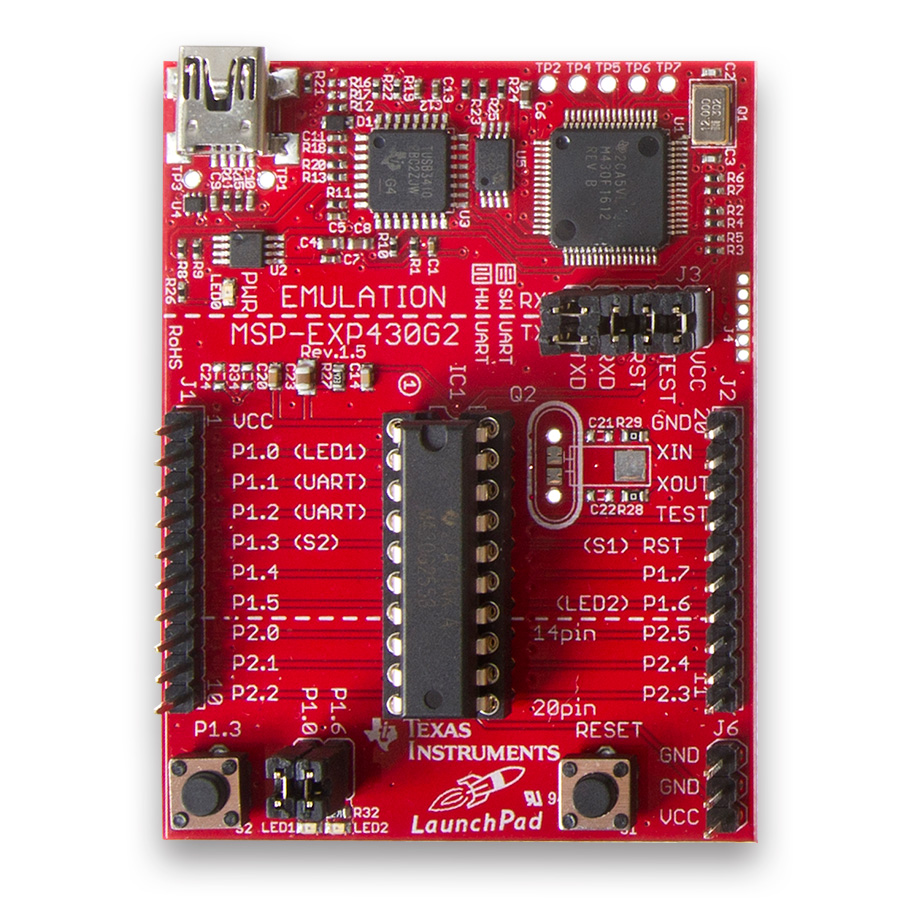
\includegraphics[scale=0.15]{launchpad-mspexp430g2.jpg}        
        \caption{The MSP-EXP430G2 dev board (ti.com)}
    \end{figure}
\end{minipage}
\end{frame}

% --- SLIDE ---
\begin{frame}[fragile]
\frametitle{MSP430 - Required tools}
\vspace{-3pt}
\begin{itemize}
    \item Required tools (assuming Debian-based linux)
\begin{codebox}
sudo apt-get install binutils-msp430 gcc-msp430 msp430-libc mspdebug
\end{codebox}
\item The code
\begin{codebox2}
#include  <msp430x20x3.h>

int main(void)
\{
    WDTCTL = WDTPW + WDTHOLD;                 // Stop watchdog timer
    P1DIR |= 0x01;                            // Set P1.0 to output direction

    for (;;)
    \{
        volatile unsigned long i;
        P1OUT ^= 0x01;                          // Toggle P1.0 using exclusive-OR
        i = 99999;                              // Delay
        do 
        \{
            i--;
        \} while (i != 0);
    \}
\}
\end{codebox2}
\codecaption{led.c}
\item \codeempha{Building} the executable
\begin{codebox}
msp430-gcc -mmcu=msp430g2553 -O0 -g led.c
\end{codebox}
\end{itemize}
\end{frame}

%%%%%%%%%%%%%%%%%%%%%%%%%%%%%%%%%%%%%%%%%%%%%%%%%%%%%%%%%%%%%%%%%%%%%%%%%%%%%%%%
\talkpart{2}{ELF And Architecture Support}
%%%%%%%%%%%%%%%%%%%%%%%%%%%%%%%%%%%%%%%%%%%%%%%%%%%%%%%%%%%%%%%%%%%%%%%%%%%%%%%%

% --- Slide ---
\begin{frame}[fragile]
\frametitle{Loading the binary}
We need to load binary sections/debug info
\begin{itemize}
    \setlength\itemsep{1em}
    \item LLDB supports \codeempha{ELF/Mach-O/PECOFF} out of the box
    \item For debugging info, DWARF is supported
    \item MSP430 compiler provides ELF with relatively good DWARF
    \item As of now
    \begin{codebox}
(lldb) file ~/led.elf
error: '~/led.elf' doesn't contain any 'host' platform 
architectures: x86_64, i386    
    \end{codebox}
    \item First step towards LLDB understanding MSP430 would be \codeempha{adding the triple}
\end{itemize}
\end{frame}

% --- Slide ---
\begin{frame}[fragile]
\frametitle{Adding the triple}
\begin{itemize}
\item Architecture and core
\begin{codebox2}
static const CoreDefinition g_core_definitions[] =
\{
    \{ eByteOrderLittle, 4, 2, 4, llvm::Triple::arm, ArchSpec::eCore_arm_generic, "arm"\},
    // ...

    // MSP430
    \codeemphb{\{ eByteOrderLittle, 2, 1, 1 , llvm::Triple::msp430 , ArchSpec::eCore_msp430, "msp430" \}}
\};

static const ArchDefinitionEntry g_elf_arch_entries[] =
\{
    // ...
    \{ ArchSpec::eCore_arm_generic, llvm::ELF::EM_ARM, LLDB_INVALID_CPUTYPE, 0xFFFFFFFFu, 0xFFFFFFFFu \},
    // ...
    \codeemphb{\{ ArchSpec::eCore_msp430, llvm::ELF::EM_MSP430, LLDB_INVALID_CPUTYPE, 0xFFFFFFFFu, 0xFFFFFFFFu \}}
\};

\end{codebox2}
\codecaption{ArchSpec.cpp}

\item From lldb:
\begin{codebox2}
(lldb) file led.elf
Current executable set to 'led.elf' (\codeemphb{msp430}).
(lldb) target list
Current targets:
* target #0: /home/user/examples/led.elf ( arch=msp430-*-*, platform=remote-linux )
\end{codebox2}
\end{itemize}
\end{frame}

% --- Slide ---
\begin{frame}[fragile]
{Architecture Support}
\begin{itemize}
\item Adding the OS (not really required)
\begin{codebox2}
bool
ArchSpec::SetArchitecture (ArchitectureType arch_type, uint32_t cpu, uint32_t sub, uint32_t os)
\{
    // ...
    switch (os)
    \{

        case llvm::ELF::ELFOSABI_GNU:     m_triple.setOS (llvm::Triple::OSType::Linux);   break;
        // MSP
        \codeemphb{case llvm::ELF::ELFOSABI_STANDALONE: m_triple.setOS (llvm::Triple::OSType::Standalone); break;}
    \}
    // ...
               
\}
\end{codebox2}
\codecaption{ArchSpec.cpp}

\item Can see the OS now
\begin{codebox2}
(lldb) target list
Current targets:
* target #0: /home/user/examples/led.elf ( arch=msp430-*-\codeemphb{standalone}, platform=remote-linux )
\end{codebox2}
\item LLDB gets the OS from EI\_OSABI in \codeempha{ELF header}
\end{itemize}
\end{frame}

% --- Slide ---
\begin{frame}[fragile]
\frametitle{Is this really enough?}
\begin{itemize}
    \setlength\itemsep{1em}
    \item To add custom ELF sections modify \codeempha{ObjectFileELF.cpp}
    \item Inspecting the ELF sections for MSP430:
\end{itemize}
\begin{codebox2}
(lldb) \codeemphb{image dump sections} led.elf
Sections for '/media/andrzej/Build/msp430/led.elf' (msp430):
  SectID     Type             File Address           File Off.  File Size  Flags      Section Name
  ---------- ---------------- ---------------------  ---------- ---------- ---------- --------------------------
  0x00000001 regular                                 0x00000000 0x00000000 0x00000000 led.elf.
  0x00000002 code             [0x000f800-0x000f89a)  0x00000094 0x0000009a 0x00000006 led.elf..text
  0x00000003 regular          [0x0000200-0x0000202)  0x0000012e 0x00000000 0x00000003 led.elf..noinit
  0x00000004 regular          [0x000ffe0-0x0010000)  0x0000012e 0x00000020 0x00000006 led.elf..vectors
  0x00000005 dwarf-aranges                           0x00000150 0x0000008c 0x00000000 led.elf..debug_aranges
  0x00000006 dwarf-info                              0x000001dc 0x00000503 0x00000000 led.elf..debug_info
  0x00000007 dwarf-abbrev                            0x000006df 0x000000f0 0x00000000 led.elf..debug_abbrev
  0x00000008 dwarf-line                              0x000007cf 0x000003a2 0x00000000 led.elf..debug_line
  0x00000009 dwarf-frame                             0x00000b72 0x00000024 0x00000000 led.elf..debug_frame
  0x0000000a dwarf-str                               0x00000b96 0x00000095 0x00000030 led.elf..debug_str
  0x0000000b dwarf-loc                               0x00000c2b 0x0000001c 0x00000000 led.elf..debug_loc
  0x0000000c dwarf-ranges                            0x00000c47 0x00000008 0x00000000 led.elf..debug_ranges
  0x0000000d regular                                 0x00000c4f 0x00000098 0x00000000 led.elf..shstrtab
  0x0000000e elf-symbol-table                        0x00000f40 0x00000720 0x00000000 led.elf..symtab
  0x0000000f regular                                 0x00001660 0x0000041a 0x00000000 led.elf..strtab
\end{codebox2}
\end{frame}

% --- Slide ---
\begin{frame}[fragile]
\frametitle{No debug info?}
\begin{itemize}
\item Inspect the line table
\begin{codebox2}
(lldb) \codeemphb{image dump line-table} led.c
warning: No source filename matched 'led.c'.
error: no source filenames matched any command arguments
\end{codebox2}
\item Inspect symbols
\begin{codebox2}
(lldb) image lookup -F main

\end{codebox2}
\item Though according to msp430-readelf, there seems to be DWARF info
\begin{codebox2}
$ \codeemphb{msp430-readelf --debug-dump=line} ~/led.elf
The File Name Table (offset 0x131):
Entry  Dir  Time  Size  Name
1      0    0     0     led.c
2      1    0     0     msp430x20x3.h
Line Number Statements:
[0x0000014c] Extended opcode 2: set Address to 0xc148
[0x00000151] Special opcode 9: advance Address by 0 to 0xc148 and Line by 4 to 5
\end{codebox2}
\end{itemize}
\end{frame}


% --- Slide ---
\begin{frame}[fragile]
\frametitle{Fixing DWARF}
C'mon LLDB, \codeempha{addresses} can be \codeempha{two bytes-wide}:
\begin{codebox2}
bool
DWARFCompileUnit::Extract(const DWARFDataExtractor &debug_info, lldb::offset_t *offset_ptr)
\{
        // ...
        bool addr_size_OK = ((m_addr_size == 4) || (m_addr_size == 8));
        // ...
\}

\end{codebox2}
\codecaption{DWARFCompileUnit.cpp}
\begin{codebox2}
bool
DWARFDebugArangeSet::Extract(const DWARFDataExtractor &data, lldb::offset_t *offset_ptr)
\{
        if ((m_header.version >= 2 && m_header.version <= 5) &&
            (m_header.addr_size == 4 || m_header.addr_size == 8) &&
            (m_header.length > 0))
\}
\end{codebox2}
\codecaption{DWARFDebugArrangeSet.cpp}
\begin{codebox2}
bool
DWARFDebugLine::ParseStatementTable(...)
\{
    // ...
    case DW_LNE_set_address:
        if (arg_size == 4)
            state.address = debug_line_data.GetU32(offset_ptr);
\}
\end{codebox2}
\codecaption{DWARFDebugLine.cpp}
\end{frame}

% --- Slide ---
\begin{frame}[fragile]
\frametitle{Fixing DWARF}
C'mon LLDB, \codeempha{addresses} can be \codeempha{two bytes-wide}:
\begin{codebox2}
bool
DWARFCompileUnit::Extract(const DWARFDataExtractor &debug_info, lldb::offset_t *offset_ptr)
\{
        // ...
        bool addr_size_OK = ((\codeemphb{m_addr_size == 2}) || (m_addr_size == 4) || (m_addr_size == 8));
        // ...
\}

\end{codebox2}
\codecaption{DWARFCompileUnit.cpp}
\begin{codebox2}
bool
DWARFDebugArangeSet::Extract(const DWARFDataExtractor &data, lldb::offset_t *offset_ptr)
\{
        if ((m_header.version >= 2 && m_header.version <= 5) &&
            (\codeemphb{m_header.addr_size == 2} || m_header.addr_size == 4 || m_header.addr_size == 8) &&
            (m_header.length > 0))
\}
\end{codebox2}
\codecaption{DWARFDebugArrangeSet.cpp}
\begin{codebox2}
bool
DWARFDebugLine::ParseStatementTable(...)
\{
    // ...
    case DW_LNE_set_address:
        if (\codeemphb{arg_size == 2})
            state.address = debug_line_data.GetU16(offset_ptr);
\}
\end{codebox2}
\codecaption{DWARFDebugLine.cpp}
\end{frame}

% --- Slide ---
\begin{frame}[fragile]
\frametitle{Fixing DWARF}
Finally, we can read the line table:
\begin{codebox}
(lldb) image dump line-table led.c
Line table for /media/andrzej/Build/msp430/led.c in `led.elf
0xf83e: /media/andrzej/Build/msp430/led.c:4
0xf844: /media/andrzej/Build/msp430/led.c:5
0xf84a: /media/andrzej/Build/msp430/led.c:6
0xf854: /media/andrzej/Build/msp430/led.c:12
0xf85e: /media/andrzej/Build/msp430/led.c:13
0xf868: /media/andrzej/Build/msp430/led.c:16
0xf87c: /media/andrzej/Build/msp430/led.c:17
\end{codebox}
... and lookup symbols:
\begin{codebox}
(lldb) image lookup -F main
1 match found in led.elf:
        Address: led.elf[0xf83e] (led.elf..text + 62)
        Summary: led.elf`main at led.c:4
\end{codebox}
\end{frame}

%%%%%%%%%%%%%%%%%%%%%%%%%%%%%%%%%%%%%%%%%%%%%%%%%%%%%%%%%%%%%%%%%%%%%%%%%%%%%%%%
\talkpart{3}{Registers}
%%%%%%%%%%%%%%%%%%%%%%%%%%%%%%%%%%%%%%%%%%%%%%%%%%%%%%%%%%%%%%%%%%%%%%%%%%%%%%%%
% --- Slide ---
\begin{frame}[fragile]
    \frametitle{Registers - lldb-server}
How does lldb-server know what are the available registers?
\begin{itemize}
\item From the Register Context
\item Used internally by lldb-server
\item Contains information on all supported registers
\item Based on information specified in \codeempha{g\_register\_infos\_<arch>[]}
\end{itemize}
For ARM,
\begin{codebox2}
static RegisterInfo g_register_infos_arm[] = \{
//  NAME     ALT     SZ   OFFSET          ENCODING          FORMAT         EH_FRAME      DWARF       
//  =======  ======= ==   ==============  ================  ============   ============= ==========  
\{   "r0",    nullptr, 4,  GPR_OFFSET(0),  eEncodingUint,    eFormatHex,  \{ ehframe_r0,   dwarf_r0, ...   \},
\{   "r1",    nullptr, 4,  GPR_OFFSET(1),  eEncodingUint,    eFormatHex,  \{ ehframe_r1,   dwarf_r1, ...   \},
\{   "r2",    nullptr, 4,  GPR_OFFSET(2),  eEncodingUint,    eFormatHex,  \{ ehframe_r2,   dwarf_r2, ...   \},
\{   "r3",    nullptr, 4,  GPR_OFFSET(3),  eEncodingUint,    eFormatHex,  \{ ehframe_r3,   dwarf_r3, ...   \},
//...
\}
\end{codebox2}
\codecaption{RegisterInfos\_arm.h}
\end{frame}

% --- Slide ---
\begin{frame}[fragile]
\frametitle{Registers - Key data strutures}
\begin{codebox}
    struct RegisterInfo
    {
        const char *name;                        // r0
        const char *alt_name;                    // can be NULL
        uint32_t byte_size;                      // 4
        uint32_t byte_offset;                    
        lldb::Encoding encoding;                 // eEncodingUint, eEncodingIEEE754
        lldb::Format format;                     // eFormatHext, eFormatFloat
        uint32_t kinds[lldb::kNumRegisterKinds]; // see below
        uint32_t *value_regs;                    // nullptr
        uint32_t *invalidate_regs;               // nullptr
    };
\end{codebox}
\codecaption{lldb-private-types.h}

\begin{codebox}
    enum RegisterKind
    {
        eRegisterKindEHFrame = 0,   // the register numbers seen in eh_frame
        eRegisterKindDWARF,         // the register numbers seen DWARF
        eRegisterKindGeneric,       // e.g. PC, SP, FP
        eRegisterKindProcessPlugin, // e.g. LLDB_INVALID_REGNUM
        eRegisterKindLLDB,          // lldb's internal register numbers
        kNumRegisterKinds
    };
\end{codebox}
\codecaption{lldb-enumerations.h}

\end{frame}

% --- Slide ---
\begin{frame}[fragile]
\frametitle{Registers - Special Registers}
Final steps: mark all the 'special' registers 
\begin{itemize}
\setbeamertemplate{itemize item}{$\Rightarrow$}
\item \codeempha{What:} eRegisterKindGeneric (field in \codeemphb{struct RegisterInfo})
\item \codeempha{Where:} g\_register\_infos\_arm[] (array in \codeemphb{RegisterInfos\_arm.h})
\end{itemize}
This is required for LLDB to know where to look for PC, SP, FP etc.

\vspace{15pt}
Possible values:
\begin{codebox}
//----------------------------------------------------------------------
// Generic Register Numbers
//----------------------------------------------------------------------
#define LLDB_REGNUM_GENERIC_PC          0   // Program Counter
#define LLDB_REGNUM_GENERIC_SP          1   // Stack Pointer
#define LLDB_REGNUM_GENERIC_FP          2   // Frame Pointer
#define LLDB_REGNUM_GENERIC_RA          3   // Return Address
...
\end{codebox}
\codecaption{lldb-defines.h}
\end{frame}

% --- Slide ---
\begin{frame}[fragile]
    \frametitle{Registers - lldb}
How does lldb know what are the available registers?
\begin{itemize}
    \item lldb-server reads RegisterContext
    \item lldb creates a RegisterContext from the info provided by lldb-server
    \item For ARM, lldb\quad \textrightarrow\quad \codeempha{\$qRegisterInfo}\quad \textrightarrow\quad lldb-server
    \item lldb-server\quad \textrightarrow\quad \codeempha{register info}\quad \textrightarrow\quad lldb
\end{itemize}
\begin{codebox}
<  18> send packet: $qRegisterInfo0#72
< 118> read packet: $name:r0;bitsize:32;offset:0;encoding:uint;format:hex;
                    set:General Purpose Registers;ehframe:0;dwarf:0;generic:arg1;#cf
<  18> send packet: $qRegisterInfo1#73
\end{codebox}
Similar situation when later reading registers:
\begin{codebox}
<  20> send packet: $p5e;thread:4cd6;#63
<  20> read packet: $00000000#00
\end{codebox}
\end{frame}

% --- Slide ---
\begin{frame}[fragile]
\frametitle{Registers - ARM read/write}
\begin{itemize}
    \setbeamertemplate{itemize item}[triangle]
    \item Carried out by lldb-server
    \item For ARM, this normally done via \codeempha{ptrace}:
\begin{codebox2}
Error
NativeRegisterContextLinux::DoReadRegisterValue(uint32_t offset,
                                                const char* reg_name,
                                                uint32_t size,
                                                RegisterValue &value)
\{
    // ...

    long data;
    Error error = NativeProcessLinux::PtraceWrapper(\codeemphb{PTRACE_PEEKUSER},
                                                    m_thread.GetID(),
                                                    reinterpret_cast<void *>(offset),
                                                    nullptr,
                                                    0,
                                                    &data);
    // ...
\}
\end{codebox2}
\codecaption{NativeRegisterContextLinux.cpp}
\item For \codeempha{register write}, replace PTRACE\_PEEKUSER with \codeempha{PTRACE\_POKEUSER}
\end{itemize}

\end{frame}

% --- Slide ---
\begin{frame}[fragile]
\frametitle{Registers - MSP430}
For MSP430, there is no lldb-server
\begin{itemize}
    \item We use mspdebug instead, which has gdb-server
    \item We cannot modify gdb-server
    \item LLDB provides an option to define registers in Python
\end{itemize}
For MSP430,
\begin{codebox2}
msp_register_infos = [
\{ 'name':'r0', 'set':0, 'bitsize':16, 'encoding':eEncodingUint, 'format':eFormatAddressInfo, 'alt-name':'pc' \},
\{ 'name':'r1', 'set':0, 'bitsize':16, 'encoding':eEncodingUint, 'format':eFormatAddressInfo, 'alt-name':'sp' \},
\{ 'name':'r2', 'set':0, 'bitsize':16, 'encoding':eEncodingUint, 'format':eFormatAddressInfo   \},
\{ 'name':'r3', 'set':0, 'bitsize':16, 'encoding':eEncodingUint, 'format':eFormatAddressInfo   \},
...
]
\end{codebox2}
\codecaption{msp430\_target\_definition.py}

\vspace{10pt}
We load registers using this command
\begin{codebox}
(lldb) settings set plugin.process.gdb-remote.target-definition-file <filename>
\end{codebox}
\end{frame}

% --- Slide ---
\begin{frame}[fragile]
\frametitle{Registers - MSP430 read/write}
\begin{itemize}
    \setbeamertemplate{itemize item}[triangle]
    \item For MSP430, \codeempha{mspdebug} does all the magic
    \item Packet exchange for MSP430:
\begin{codebox}
(lldb) register read
<   7> send packet: $Hg1#e0
<   1> read packet: +
<   4> read packet: $#00
<   1> send packet: +
<   5> send packet: $g#67
<   1> read packet: +
<  68> read packet: $78f87c02030000008202ff5a0000000000000...0000000#3a
<   1> send packet: +
General Purpose Registers:
        r0 = 0xf878  led.elf`main + 58
        r1 = 0x027c
        r2 = 0x0003
        r3 = 0x0000
        r4 = 0x0282
        r5 = 0x5aff
           ...
\end{codebox}
\end{itemize}
\end{frame}

%%%%%%%%%%%%%%%%%%%%%%%%%%%%%%%%%%%%%%%%%%%%%%%%%%%%%%%%%%%%%%%%%%%%%%%%%%%%%%%%
\talkpart{4}{Memory and Breakpoints}
%%%%%%%%%%%%%%%%%%%%%%%%%%%%%%%%%%%%%%%%%%%%%%%%%%%%%%%%%%%%%%%%%%%%%%%%%%%%%%%%
% --- Slide ---
\begin{frame}[fragile]
\frametitle{Memory}
\begin{itemize}    
    \setlength\itemsep{1em}
    \setbeamertemplate{itemize item}[triangle]
    \item Carried out by the \codeempha{lldb-server}
    \item Very well defined in the Linux environment (e.g. for ARM):
\begin{codebox2}
Error
NativeProcessLinux::ReadMemory (...)
\{
    // ... 
    for (bytes_read = 0; bytes_read < size; bytes_read += remainder)
    \{
        Error error = NativeProcessLinux::PtraceWrapper(\codeemphb{PTRACE_PEEKDATA},
                                                        GetID(),
                                                        (void*)addr,
                                                        nullptr,
                                                        0,
                                                        &data);
       ...
\}

\end{codebox2}
\codecaption{NativeProcessLinux.cpp}
\item For memory write, replace PTRACE\_PEEKDATA with \codeempha{PTRACE\_POKEDATA}
\end{itemize}
\end{frame}

% --- Slide ---
\begin{frame}[fragile]
\frametitle{Memory}
\begin{itemize}
    \setlength\itemsep{1em}
    \setbeamertemplate{itemize item}[triangle]
    \item For MSP430, we only care about the packets:
    \begin{codebox}
(lldb) memory read 0x800
<  12> send packet: $m800,200#c3
<   1> read packet: +
 <1028> read packet: $ffffffffffffffffffffffff...ffffffffffffffff#00
<   1> send packet: +
0x00000800: ff ff ff ff ff ff ff ff ff ff                    ..........

    \end{codebox}
    \vspace{10pt}
    \item So, assuming there's nothing special about your memory architecture...
    \item Hint: extensive data formatting takes place in \codeemphb{DataExtractor.cpp}
\end{itemize}
\end{frame}

% --- Slide ---
\begin{frame}[fragile]
\frametitle{Breakpoints - Overview}
\begin{tikzpicture}
  % \node[draw=uipurple,rounded corners = 1pt, fill=uidarkgray,text=white, line width=1.5pt, ] (process-starts) at (15,3) {User process};
  \node[draw=white,rounded corners = 1pt, fill=white,text=uidarkgray, line width=1.5pt, ] (process-starts) at (15,3) {User process};
  \node[draw=white,rounded corners = 1pt, fill=white,text=uidarkgray, line width=1.5pt, ] (os-lldb) at (20,3) {lldb-server (via ptrace)};
  \node[draw=uipurple,rounded corners = 1pt, fill=uidarkgray,text=white, line width=1.5pt, ] (break) at (15,1) {break};
  \node[draw=uipurple,rounded corners = 1pt, fill=uidarkgray,text=white, line width=1.5pt, ] (break-handler-starts) at (20,1) {\tiny SIGTRAP handling starts};
  \node[draw=uipurple,rounded corners = 1pt, fill=uidarkgray,text=white, line width=1.5pt, ] (break-handler-ends) at (20,0) {\tiny SIGTRAP handling ends};
  % \node[draw=uipurple,rounded corners = 1pt, fill=uidarkgray,text=white, line width=1.5pt, ] (process-ends) at (15,-1) {Process ends};
  \node[draw=white,rounded corners = 1pt, fill=white, line width=1.5pt, ] (process-ends) at (15,-1) {};

  % \node[] (start) at (13,3.5) {};
  % \node[] (end) at (13,-1.5) {};
  \node[] (start) at (13,3) {};
  \node[] (end) at (13,-1) {};
  
  \draw[->] (process-starts) to (break) [line width=1.5pt];
  \draw[->] (break) to (process-ends) [line width=1.5pt];
  \draw[->] (break-handler-starts) to (break-handler-ends) [line width=1.5pt];
  \draw[->] (break) to node[midway, above] {\tiny SIGTRAP }(break-handler-starts) [dashed, line width=1pt];
  \draw[->] (break-handler-ends) to node[midway, below, sloped] {\tiny ptrace returns control }(break) [dashed, line width=1pt];
  \draw[->] (start) to node[midway, sloped, below] {\tiny Execution (ptrace'd)}(end) [line width=0.5pt];
  
  \node at (16, -2.0) {\textit{Exceptional Control Flow - Traps}};
\end{tikzpicture}

\begin{itemize}
    \item On Linux, break/trap instruction raises \codeempha{SIGTRAP}
    \item SIGTRAP normally  indicates a \codeempha{breakpoint}
    \item ptrace \codeempha{intercepts all signals} (apart from SIGKILL) sent to its tracee
\end{itemize}
\end{frame}

% --- Slide ---
\begin{frame}[fragile]
\frametitle{Breakpoints - Setting a breakpoint with ptrace}

\begin{codebox2}
Error
SoftwareBreakpoint::CreateSoftwareBreakpoint (...)
\{
    // ...
    Error error = process.\codeempha{GetSoftwareBreakpointTrapOpcode} (size_hint, bp_opcode_size, bp_opcode_bytes);

    // ...
    // Enable the breakpoint.
    uint8_t saved_opcode_bytes [MAX_TRAP_OPCODE_SIZE];
    error = \codeempha{EnableSoftwareBreakpoint} (process, addr, bp_opcode_size, bp_opcode_bytes, saved_opcode_bytes);
    //...
\}

Error
SoftwareBreakpoint::EnableSoftwareBreakpoint (...)
\{
    // ...
    // Save the original opcodes by reading them so we can restore later.
    size_t bytes_read = 0;

    Error error = process.\codeempha{ReadMemory}(addr, saved_opcode_bytes, bp_opcode_size, bytes_read);
 
    // ...
    // Write a software breakpoint in place of the original opcode.
    size_t bytes_written = 0;
    error = process.\codeempha{WriteMemory}(addr, bp_opcode_bytes, bp_opcode_size, bytes_written);
    // ...
\}
\end{codebox2}
\codecaption{SoftwareBreakpoint.cpp}
\end{frame}


% --- Slide ---
\begin{frame}[fragile]
\frametitle{Breakpoints - opcodes}
\begin{itemize}
    \item Most architectures offer a special \codeempha{break instruction}
    \item LLDB needs the corresponding \codeempha{op-code}
\end{itemize}
\begin{codebox}
Error
NativeProcessLinux::GetSoftwareBreakpointTrapOpcode (size_t trap_opcode_size_hint,
                                                     size_t &actual_opcode_size,
                                                     const uint8_t *&trap_opcode_bytes)
{
    // ...
    static const uint8_t g_aarch64_opcode[] = { 0x00, 0x00, 0x20, 0xd4 };
    static const uint8_t g_arm_breakpoint_opcode[] = { 0xf0, 0x01, 0xf0, 0xe7 };
    static const uint8_t g_i386_opcode [] = { 0xCC };
    static const uint8_t g_mips64_opcode[] = { 0x00, 0x00, 0x00, 0x0d };
    static const uint8_t g_mips64el_opcode[] = { 0x0d, 0x00, 0x00, 0x00 };
    static const uint8_t g_thumb_breakpoint_opcode[] = { 0x01, 0xde };
    //...
}
\end{codebox}
\codecaption{NativeProcessLinux.cpp}
\begin{itemize}
    \item For MSP430, this is not required (not using lldb-server)
\end{itemize}
\end{frame}

% --- Slide ---
\begin{frame}[fragile]
\frametitle{Breakpoints - MSP430}
Adding 'op-code' for MSP430:
\begin{codebox2}
size_t
PlatformLinux::GetSoftwareBreakpointTrapOpcode (Target &target,
                                                BreakpointSite *bp_site)
\{
    ArchSpec arch = target.GetArchitecture();
    const uint8_t *trap_opcode = NULL;
    size_t trap_opcode_size = 0;

    switch (arch.GetMachine())
    \{
    default:
        assert(false && "CPU type not supported!");
        break;

    // ...
    case \codeemphb{llvm::Triple::msp430}:
        \{
            static const uint8_t g_msp430_opcode[] = { 0x43, 0x43 };
            trap_opcode = g_msp430_opcode;
            trap_opcode_size = sizeof(g_msp430_opcode);
        \}
        break;
    // ...
\}
\end{codebox2}
\codecaption{PlatformLinux.cpp}
\end{frame}

% --- Slide ---
\begin{frame}[fragile]
\frametitle{Breakpoints - Step-by-step}
\begin{itemize}
    \setbeamertemplate{itemize item}[triangle]
\item \codeempha{Setting} the breakpoint (lldb):
        \begin{codebox}
(lldb) breakpoint set -n main
Breakpoint 1: where = led.elf`main + 6 at led.c:5, address = 0xf844
        \end{codebox}
    \item \codeempha{Resolving} the breakpoint and sending the corresponding packet (lldb):
        \begin{codebox}
<  13> send packet: $Z0,f844,2#48
<   1> read packet: +
<   6> read packet: $OK#9a
        \end{codebox}
    \item \codeempha{Overwritting the opcode} (lldb-server/mspdebug)
    \item \codeempha{Hitting the breakpoint} (lldb-server/mspdebug \textrightarrow lldb):
\begin{codebox2}
< 135> read packet: $T0500:44f8;01:7c02;02:0100;03:0000;04:8202;05:ff5a;06:0000;07:0000;08:0000;09:0000;
0a:0000;0b:0000;0c:0000;0d:0000;0e:0000;0f:0000;#9c
    ...
Process 1 stopped
* thread #1: tid = 0x0001, 0xf844 led.elf`main + 6 at led.c:5, stop reason = breakpoint 1.1
    frame #0: 0xf844 led.elf`main + 6 at led.c:5
\end{codebox2}
\end{itemize}
\end{frame}

% --- Slide ---
\begin{frame}[fragile]
\frametitle{Breakpoints - Summary}
Finally (provided that we have debug information):
\begin{codebox2}
(lldb) \codeempha{breakpoint set} --file led.c --line 16
(lldb) \codeempha{continue}
Process 1 resuming
Process 1 stopped
* thread #1: tid = 0x0001, 0xf868 led.elf`main + 42 at led.c:16, stop reason =
breakpoint 1.1
    frame #0: 0xf868 led.elf`main + 42 at led.c:16
   13           i = 99999;                              // Delay
   14           do 
   15           \{
-> 16               i--;
   17           \} while (i != 0);
   18       \}
   19   \}
(lldb) \codeempha{next}
Process 1 stopped
* thread #1: tid = 0x0001, 0xf87c led.elf`main + 62 at led.c:17, stop reason = step over
    frame #0: 0xf87c led.elf`main + 62 at led.c:17
   14           do 
   15           \{
   16               i--;
-> 17           \} while (i != 0);
   18       \}
   19   \}
\end{codebox2}
\end{frame}

%%%%%%%%%%%%%%%%%%%%%%%%%%%%%%%%%%%%%%%%%%%%%%%%%%%%%%%%%%%%%%%%%%%%%%%%%%%%%%%%
\talkpart{5}{Other Key Features}
%%%%%%%%%%%%%%%%%%%%%%%%%%%%%%%%%%%%%%%%%%%%%%%%%%%%%%%%%%%%%%%%%%%%%%%%%%%%%%%%

% --- Slide ---
\begin{frame}[fragile]
\frametitle{ABI - Overview}
Implemented as part of the LLDB ABI plugin
\begin{itemize}
    \item Based on the \codeempha{calling convention} for the architecture
    \item ABI plugin also tells LLDB about callee-saved and caller-saved registers
    \item Much easier when a stack and \codeempha{frame pointer}, or CFI is available
\end{itemize}
What's CFI?
\begin{itemize}
    \item Call Frame Information
    \item Generated by the compiler and available in DWARF
    \item LLDB uses info from .eh\_frame
\end{itemize}
For MSP430
\begin{itemize}
    \item Don't have frame pointer or CFI
    \item The \codeempha{return address} is pushed on to the stack
\end{itemize}
\end{frame}

% --- Slide ---
\begin{frame}[fragile]
\frametitle{ABI - MSP430}
We implemented an experimental MSP430 ABI, \codeempha{ABISysV\_msp430}
\begin{itemize}   
\item Example:
    \begin{codebox}
(lldb) bt
* thread #1: tid = 0x0001, 0xc15e a.out`calc2(y=22) + 6 at led.c:11,
stop reason = signal SIGTRAP
  * frame #0: 0xc15e a.out`calc2(y=22) + 6 at led.c:11
    frame #1: 0xc154 a.out`calc1(x=22) + 12 at led.c:6
    \end{codebox}
    \item The two frames listed are correct
    \item However, the variable values are incorrect
    \item Unwinding to the main function is not being done yet    
\end{itemize}
Our temporary solution for now
\begin{itemize}
    \item Set the PC to be SP + 2
    \item This would \codeempha{only work} for functions with one argument!
    \item Have to investigate this further
\end{itemize}
\end{frame}

% --- Slide ---
\begin{frame}[fragile]
\frametitle{ABI - ARM}
For ARM,
\begin{itemize}
    \item Start by implementing CreateDefaultUnwindPlan(), specifying offsets to the PC, FP, based on the CFA
    \begin{codebox}
bool
ABISysV_arm::CreateDefaultUnwindPlan (UnwindPlan &unwind_plan)
{
    uint32_t fp_reg_num = dwarf_r11;
    uint32_t pc_reg_num = dwarf_pc;
    // ...
    row->GetCFAValue().SetIsRegisterPlusOffset (fp_reg_num, 2 * ptr_size);
    row->SetRegisterLocationToAtCFAPlusOffset(fp_reg_num, ptr_size * -2, true);
    row->SetRegisterLocationToAtCFAPlusOffset(pc_reg_num, ptr_size * -1, true);
    unwind_plan.AppendRow (row);
    unwind_plan.SetSourceName ("arm default unwind plan");
    // ...
}
    \end{codebox}
    \codecaption{ABISysV\_arm.cpp}
    \item This info is used to locate the values to be stored into the respective registers, and for \codeempha{unwinding the stack}
\end{itemize}
\end{frame}

% --- Slide ---
\begin{frame}[fragile]
\frametitle{Expression Evaluation}
\begin{itemize}
    \item Without implementing any code, we already have \codeempha{simple expression evaluation} for MSP430
    \begin{codebox}
(lldb) expr y
(int) $4 = 2200
(lldb) expr &y
(int *) $5 = 0x03e6
(lldb) expr y = y * 10
(int) $6 = 22000
(lldb) memory read 0x3e6 -f d -s 2
0x000003e6: 22000
    \end{codebox}
    \item LLDB uses Clang for parsing, and performs \codeempha{IR interpretation}
    \item For expression evaluation to work properly, please use the latest MSP430 compiler from TI
    \begin{itemize}
    \item \href{http://www.ti.com/tool/msp430-gcc-opensource}{\nolinkurl{www.ti.com/tool/msp430-gcc-opensource}}
    \end{itemize}
    \item Future work for MSP430 would be to support calling functions existing in the binary from IR, by implementing \codeempha{PrepareTrivialCall()} in the ABI
\end{itemize}
\end{frame}

% --- Slide ---
\begin{frame}[fragile]
\frametitle{Expression Evaluation - Behind the scenes}
    \begin{codebox2}
void $__lldb_expr(void *$__lldb_arg) 
\{ 
    \codeemphb{y = y * 10;}
\}
    \end{codebox2}
    \begin{codebox2}
target datalayout = "e-m:e-p:16:16-i32:16:32-a:16-n8:16"
target triple = "msp430--"

define void @"_Z12$__lldb_exprPv"(i8* %"$__lldb_arg") #0 \{
entry:
%0 = getelementptr i8, i8* %"$__lldb_arg", i32 8
%1 = bitcast i8* %0 to i16**
%2 = getelementptr i8, i8* %"$__lldb_arg", i32 0
%3 = bitcast i8* %2 to i16**
%"$__lldb_arg.addr" = alloca i8*, align 2, !clang.decl.ptr !5
store i8* %"$__lldb_arg", i8** %"$__lldb_arg.addr", align 2
%guard.uninitialized = icmp eq i8 0, 0
br i1 %guard.uninitialized, label %init.check, label %init.end

init.check:
         ; preds = %entry
  %4 = load i16*, i16** %1, align 2
  %5 = load i16, i16* %4, align 2
  \codeemphb{%mul = mul i16 %5, 10}
  %6 = load i16*, i16** %1, align 2
  store i16 %mul, i16* %6, align 2
  store i16* %6, i16** %3, align 2
  br label %init.end
// ...\}
    \end{codebox2}
\end{frame}

% --- Slide ---
\begin{frame}[fragile]
\frametitle{Disassembly}
\begin{itemize}
    \item LLDB leverages the \codeempha{disassembler from LLVM}
    \item MSP430 doesn't have a disassembler yet implemented in LLVM
    \begin{codebox2}
(lldb) dis
error: Unable to find Disassembler plug-in for the 'msp430' architecture.
    \end{codebox2}
    \item For ARM,
    \begin{codebox2}
DisassemblerLLVMC::DisassemblerLLVMC (\ldots)
\{
    //...
    const char *triple = arch.GetTriple().getTriple().c_str();
    ArchSpec thumb_arch(arch);
    if (arch.GetTriple().getArch() == llvm::Triple::arm)\{
        std::string thumb_arch_name (thumb_arch.GetTriple().getArchName().str());
        // ...
        thumb_arch_name.insert(0, "thumb");
    \}
    thumb_arch.GetTriple().setArchName(llvm::StringRef(thumb_arch_name.c_str()));
    // ...
    \codeemphb{m_disasm_ap.reset (new LLVMCDisassembler(triple, cpu, features_str.c_str()));}
    std::string thumb_triple(thumb_arch.GetTriple().getTriple());
    m_alternate_disasm_ap.reset(new LLVMCDisassembler(thumb_triple.c_str()));
\}

    \end{codebox2}
    \codecaption{DisassemblerLLVMC.cpp}
\end{itemize}
\end{frame}

% --- Slide ---
\begin{frame}[fragile]
\frametitle{Single-stepping}
\begin{itemize}
    \item PTRACE\_SINGLESTEP tells the kernel to stop at every instruction
    \begin{codebox2}
NativeProcessLinux::SingleStep(lldb::tid_t tid, uint32_t signo)\{
    //...
    // If hardware single-stepping is not supported, we just do a continue. The breakpoint on the
    // next instruction has been setup in NativeProcessLinux::Resume.
    return PtraceWrapper(SupportHardwareSingleStepping() ? \codeemphb{PTRACE_SINGLESTEP} : \codeemphb{PTRACE_CONT},
            tid, nullptr, (void*)data);
\}

    \end{codebox2}
    \codecaption{NativeProcessLinux.cpp}
    \item For MSP430, LLDB sends the \codeempha{s RSP packet} to request mspdebug to step
    \begin{codebox2}
Process 1 stopped
* thread #1: tid = 0x0001, \codeemphb{0xc164} a.out`calc2(y=22000) + 12 at led.c:12,
stop reason = step in
    frame #0: 0xc164 a.out`calc2(y=22000) + 12 at led.c:12
   9  int calc2(int y)
   10 {
   11     return 10 + y ;
-> 12 }
(lldb) s
< 5> send packet: \codeemphb{$s#73}
< 1> read packet: +
< 135> read packet: $T0500:\codeemphb{66c1};01:ec03;02:0000;03:0000;04:04c0;05:04c0;06:0200;07:0000;08:ffff;09:9886;
0a:0100;0b:0302;0c:6e00;0d:9886;0e:0100;0f:0400;#e2
< 1> send packet: +
    \end{codebox2}
\end{itemize}
\end{frame}

%%%%%%%%%%%%%%%%%%%%%%%%%%%%%%%%%%%%%%%%%%%%%%%%%%%%%%%%%%%%%%%%%%%%%%%%%%%%%%%%
\talkpart{6}{Debugging Tips}
%%%%%%%%%%%%%%%%%%%%%%%%%%%%%%%%%%%%%%%%%%%%%%%%%%%%%%%%%%%%%%%%%%%%%%%%%%%%%%%%

% --- Slide ---
\begin{frame}[fragile]
\frametitle{Debugging Tips}
LLDB logs provide detailed information
\begin{itemize}
    \item log enable \textless log-channel\textgreater  \textless log-category\textgreater
    \item There are many channels and categories available
    \begin{codebox2}
(lldb) \codeemphb{log list}
Logging categories for 'gdb-remote':
  packets - log gdb remote packets
  memory - log memory reads and writes
Logging categories for 'lldb':
  break - log breakpoints  
  dyld - log shared library related activities
  expr - log expressions    
    \end{codebox2}
    \item \codeempha{log enable gdb-remote packets}
    \begin{itemize}
        \item Shows all RSP communication, very useful for debugging
        \item Can separate lldb and lldb-server
    \end{itemize}
    \item \codeempha{log enable lldb unwind}
    \begin{itemize}
        \item useful for tracing unwinding problems
    \end{itemize}
\end{itemize}
\end{frame}

% --- Slide ---
\begin{frame}[fragile]
\frametitle{Debugging Tips}
Sending a single RSP packet
\begin{itemize}
    \item \codeempha{process plugin packet send}
    \item Very useful to isolate lldb and lldb-server
    \begin{codebox}
(lldb) process plugin packet send g
packet: g
response: 54c1ee030000000004c004c001000000ffff9886010003026e00988601000400
(lldb) process plugin packet send ?
packet: ?
response: T0500:54c1;01:ee03;02:0000;03:0000;04:04c0;05:04c0;06:0100
;07:0000;08:ffff;09:9886;0a:0100;0b:0302;0c:6e00;0d:9886;0e:0100;0f:0400;
    \end{codebox}
\end{itemize}
Enabling lldb-server logs
\begin{itemize}
\begin{codebox}
$ lldb-server g --log-file /dev/tty --log-channels "lldb all:gdb-remote all"
localhost:1234 ~/arm_binary.out
\end{codebox}
\end{itemize}
\end{frame}

% --- Slide ---
\begin{frame}[fragile]
\frametitle{Debugging Tips}
\begin{itemize}
    \item Make sure both LLDB and executable are built in  \codeempha{debug mode}
    \item Use dwarfdump to \codeempha{verify DWARF} generated for the executable is proper
    \begin{itemize}
        \item For MSP430, due to LLDB parsing DWARF wrongly, couldn't see source file/line numbers
    \end{itemize}
    \item Use \codeempha{image dump sections} command to make sure sections have been loaded properly
    \item Use \codeempha{objdump/readelf} to
    \begin{itemize}
        \item Check disassembly
        \item Verify ELF header
    \end{itemize}
    \item Use \codeempha{strace} for debugging signals
    \item Use \codeempha{GDB} to compare debugging sessions
    \begin{itemize}
        \item For MSP430, we used \codeempha{msp430-gdb} for reference
    \end{itemize}
\end{itemize}
\end{frame}

% --- Slide ---
%\begin{frame}[fragile]
%\frametitle{Runtime Design Tips}
%\begin{itemize}
%    \item If you have a simulator, might be useful to think of incorporating lldb-server functionality along with it
%    \item Design the runtime keeping debugging in mind to have a good debug API
%\end{itemize}
%\end{frame}

%%%%%%%%%%%%%%%%%%%%%%%%%%%%%%%%%%%%%%%%%%%%%%%%%%%%%%%%%%%%%%%%%%%%%%%%%%%%%%%%
\talkpart{7}{MSP430 Quick Recap}
%%%%%%%%%%%%%%%%%%%%%%%%%%%%%%%%%%%%%%%%%%%%%%%%%%%%%%%%%%%%%%%%%%%%%%%%%%%%%%%%

% --- Slide ---
\begin{frame}[fragile]
\frametitle{MSP430 Quick Recap}
Steps for implementing support for MSP430 in LLDB:
\begin{itemize}
    \setbeamertemplate{itemize item}[triangle]
    \setlength\itemsep{0.75em}
    \item msp430 \codeempha{triple} to LLDB
    \item Describe msp430 \codeempha{registers} in a python file
    \item Fix \codeempha{DWARF} parsing errors in LLDB
    \item Added msp430 \codeempha{breakpoint opcode} to LLDB
    \item Implemented msp430 \codeempha{ABI}
\end{itemize}
Very useful links:
\begin{itemize}
    \setlength\itemsep{0.75em}
    \item binutils - 
    \href{http://www.ti.com/tool/msp430-gcc-opensource}{\nolinkurl{www.ti.com/tool/msp430-gcc-opensource}}
    \item mspdebug - 
    \href{http://dlbeer.co.nz/mspdebug/}{\nolinkurl{dlbeer.co.nz/mspdebug/}}
\end{itemize}
\end{frame}

% --- Slide ---
\begin{frame}[fragile]
\frametitle{MSP430 Quick Recap}
    \begin{codebox2}
$ \codeemphb{./mspdebug sim}
MSPDebug version 0.23 - debugging tool for MSP430 MCUs
(mspdebug) $ \codeemphb{prog ~/led.elf}
Erasing...
Programming...
Writing    2 bytes at fffe [section: __reset_vector]...
Writing   16 bytes at c000 [section: .rodata]...
Writing  804 bytes at c010 [section: .text]...
Writing    4 bytes at c334 [section: .data]...
Done, 826 bytes total
(mspdebug) $ \codeemphb{gdb}
Bound to port 2000. Now waiting for connection...
    \end{codebox2}
    \begin{codebox2}
(lldb) \codeemphb{file /media/andrzej/Build/msp430/led.elf}
Current executable set to '/media/andrzej/Build/msp430/led.elf' (msp430).
(lldb) \codeemphb{settings set plugin.process.gdb-remote.target-definition-file msp430_target_definition.py}
(lldb) \codeemphb{b main}
Breakpoint 1: where = led.elf`main + 6 at led.c:5, address = 0xf844
(lldb) gdb-remote 2000
Process 1 stopped
* thread #1: tid = 0x0001, 0xf844 led.elf`main + 6 at led.c:5, stop reason = breakpoint 1.1
    frame #0: 0xf844 led.elf`main + 6 at led.c:5
   2   
   3    int main(void)
   4    \{
-> 5        WDTCTL = WDTPW + WDTHOLD;
(lldb)
    \end{codebox2}
\end{frame}
